\cotefile{77}
\scanpage{18}
Quant aux formes quadratiques invariantes \inserted{quasi-inv.} sur
l'espace des translations $\check V$ (toujours sous l'hyp.
$\alpha^2-4$ inv) elles sont comprises parmi les
\unsure{quasi-invar.|quasi-inva.|quasi-inv.} sur \unsure{$\widetilde E$|$t^{=}$|$\check E$} (dont \inserted{\deleted{\unsure{l'invariance pour}}\deleted{\unsure{une certaine}} puisque $\alpha\ne2$ fibre par fibre est un} quotient $\unsure{\}|)}$,
on trouve donc, si $\alpha$ inv., les multiples
seulement de la forme $xy$ (qui est non
dégénérée et donne lieu à la conique circonscrite
à $P$), et si $\alpha=0$ i.e. \deleted{\unsure{que}}
${\zeta}^2=-1$ \inserted{(donc $2$ inv. sur $S$)}, on trouve comme dessus \deleted{les}
multiples de $x^2+y^2$ et de $x^2-y^2$, dont
la \deleted{\unsure{deuxième devant prendre les mêmes valeurs}}\inserted{première prend les valeurs}
$1+1=2$ et $\zeta^2+{\zeta'}^2=\alpha^2-2=-2$ sur les sommets
de $P$ \inserted{(donc deux valeurs distinctes)}, et la deuxième y prend la valeur $0$,
mais (comme nous avons remarqué) définit une
conique circonscrite dégénérée\ldots .

\begin{center}\rule{1.6cm}{0.3pt}\end{center}

Il reste à étudier la question des formes
quadratiques \inserted{quasi-}invariantes, d'abord pour $\alpha=2$
et $\alpha=-2$, puis éventuellement pour $\alpha$
``variable'' général\unsure{?}\ldots .

% archive sheet number: 17

\scanpage{19}
Coniques circonscrites à un polygone \unsure{regulier|régulier}.

Faisons les calculs en coordonnées \unsure{universelle|universelles}

\[
\left\{\begin{aligned}
s_0&=(0,0)\\
s_1&=(1,0)\\
s_{-1}&=(0,1)\\
s_2&=(1+\alpha,1)\\
s_{-2}&=(1,1+\alpha)
\end{aligned}\right. \tag*{(1)}
\]

Écrivons une fonction quadratique \unsure{général|générale} en coord. affines
\[
q(x,y)=ax^2+bxy+cy^2+ux+vy+d
\]
\deleted{\unsure{pour}} Écrivons que \deleted{\unsure{le lieu}} la conique qu'elle définit
passe par les \inserted{5 pts} $s_i$, $-2\le i\le +2$ ; on trouve

\[
\left.\begin{aligned}
q(s_0)&=d=0\\
q(s_1)&=a+u=0&\text{i.e. }u&=-a\\
q(s_{-1})&=\deleted{\unsure{b}}\unsure{c|b}+v=0&\text{--- }\ v&=-b
\end{aligned}\right\}
q(x,y)=a(x^2-x)+c(y^2-y)+bxy\quad\deleted{\unsure{+c}}
\]

\[
\left\{\begin{aligned}
q(s_2)&=a(1+\alpha)\alpha+b(1+\unsure{2|\alpha})=(1+\alpha)(\alpha a+b)=0\\
q(s_{\unsure{1|-2}})&=\deleted{\unsure{b}}c(1+\alpha)\alpha+b(1+\alpha)=(1+\alpha)(\alpha\deleted{\unsure{b}}c+b)=0
\end{aligned}\right.
\]

Si $\alpha-1$ inv. (i.e. on n'a de triangle sur aucune fibre
la condition s'écrit
\[
 b=-\alpha a\inserted{\unsure{=}}\deleted{\underbrace{\unsure{,\,a=-\alpha b}}}\,=-\alpha c
\]
ou encore

et si $\alpha$ inversible (i.e. on n'a pas de carrés sur aucune fibre)
\[
 a=c,\quad b=-\alpha a,\quad \unsure{''}
\]
donc $q$ doit être multiple \inserted{$a q_0$} de la forme
\[
q_0(x,y)=(x^2-x)+(y^2-y)-\alpha xy \tag*{(2)}
\]
% slanted
\margin{\uline{NB} C'est la normalisation pour laquelle $q(s-s')=1$ si $s,s'$ sont 2 sommets consécutifs \unsure{de $P$|$(P)$} \ldots}

Comme celle-ci est invariante sous $G$, la

% archive sheet number: 18

\scanpage{20}
\deleted{b) celui qui correspond au plan $(x,y$}

\unsure{Plan Tangent|Plan tangent} : $C$ le long de $D_{\zeta}$

Son équation est (utilisant la matrice
adjointe \deleted{$\unsure{x,y,z}$} $\Delta$) :
\[
Ax+By+Cz=0
\]
\[
\deleted{2x-\alpha y=}
\]
où $A,B,C$ sont donnés par $\Delta\cdot(1,\zeta,0)$ i.e.
\[
\begin{aligned}
 A&=2-\alpha\zeta\deleted{\unsure{0}}, & B&=-\unsure{\zeta}\alpha+2\zeta, & C&=-(1+\zeta)\\
 &=1-\zeta^2\deleted{=\unsure{\zeta(\zeta'-\zeta)}}&&=\zeta-\zeta^{-1}=-\zeta^{-1}(1-\zeta^2)\\
 &=(1-\zeta)(1+\zeta)&&=-\zeta^{-1}(1-\zeta)(1+\zeta)
\end{aligned}
\]
On peut (comme $1+\zeta$ \deleted{\unsure{$=2$}} inv. i.e. $\zeta=-1$ fibre par
fibre i.e. $\alpha\ne-2$ fibre par fibre, par hyp.) \unsure{simplifier|diviser}
par $(1+\zeta)$, on trouve l'équation
\[
H_\zeta:\quad\left\{\begin{aligned}
 (1-\zeta)x-\zeta^{-1}(1-\zeta)y-z&=0\qquad\text{i.e.}\\
 z&=(1-\zeta)(x-\zeta^{-1}y)
\end{aligned}\right.
\]
\diagram{\begin{tikzcd}[ampersand replacement=\&,column sep=small,row sep=small]
D_\zeta \& {\subset H_\zeta} \& {\subset E}\\
\& V\arrow[u,"\unsure{\sim|\simeq}"'] \&
\end{tikzcd}}

Ainsi $C$ s'identifie à la \inserted{clôture projective de} \unsure{l'espace|espace} affine
associé à l'extension de $E/H_\zeta$ par $H_\zeta/D_\zeta\simeq V/D_\zeta\simeq$

Comme l'axe des $z$ \inserted{$(\underline{O}_S e_3)$} est un supplémentaire,
\unsure{icette|ledit} \inserted{espace affine est} \deleted{un} \uline{vectoriel}, isomorphe au fibré
vectoriel cov. associé :
\[
{\underbrace{(E/H_\zeta)}_{\underline{O}_S\cdot e_3}}^{\otimes-1}\otimes
\underbrace{H_\zeta/D_\zeta}_{\simeq\underline{O}_S e_1}
\]

\figure{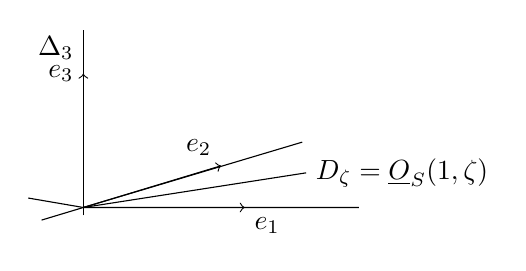
\begin{tikzpicture}[x=1cm,y=1cm]
\draw (-.70,.12)--(0,0)--(3.5,0);
\draw[->] (0,0)--(2.05,0) node[below right] {$e_1$};
\draw (0,-.10)--(0,2.25);
\draw[->] (0,0)--(0,1.7) node[left] {$e_3$};
\node[left] at (0,2.02) {$\unsure{\Delta_3}$};
\draw (-.53,-.16)--(0,0)--(2.78,.83);
\draw[->] (0,0)--(1.75,.53) node[above left] {$e_2$};
\draw (0,0)--(2.83,.44) node[right] {$D_\zeta=\underline{O}_S(1,\zeta)$};
\end{tikzpicture}}

% archive sheet number: 19

\scanpage{21}
Extensions quadratiques

\unsure{(43 p)|43 p)}

% archive sheet number: 20

\scanpage{22}
Extensions quadratiques.

1. Un \deleted{\unsure{schéma}}\inserted{revêtement} quadratique d'un schéma $S$ est un
$S$-schéma $\Omega$ fini loc. libre de rang 2 sur $S$. La catégorie
de ces revêtements quadratiques (sur $S$ fixé) est
équivalente à celle des $\underline{O}_S$-Algèbres (comm. unifères)
\inserted{$B$} loc. libres de rang 2, ou \inserted{dites aussi} extensions quadratiques
de $\underline{O}_S$. Pour $S$ variable, on trouve une catégorie
fibrée sur $(\mathrm{Sch})_{/S}$
\[
\Omega=\operatorname{Spec}(B) \tag*{(1)}
\]
Soit \deleted{\unsure{le}}
\[
\check L=B/\underline{O}_S\qquad 0\mathbin{-}\underline{O}_S\xrightarrow{i}B\mathbin{-}\check L\longrightarrow0 \tag*{(2)}
\]
module inversible. On a une structure d'extension
\[
0\mathbin{-}L^{\deleted{\unsure{\vee}}}\longrightarrow\check B\xrightarrow{\pi}\underline{O}_S\mathbin{-}0 \tag*{(3)}
\]
i.e. un fibré affine de \unsure{rg|rang} 1 sur $S$, ayant
$L^{\deleted{\unsure{\vee}}}$ comme module des translations, \deleted{les splittings}\deleted{scindages}
soit
\[
\begin{aligned}
 E&\subset\check{\mathbb V}(\check B)\simeq\mathbb V(B)=\operatorname{Spec}(\underline{\mathrm{Sym}}_{\underline{O}_S}(B))\\
 \Vert&\\[-3pt]
 \operatorname{Spec}(&\underline{\mathrm{Sym}}_{\underline{O}_S} B/(e_B-1))
\end{aligned} \tag*{(4)}
\]
où $e$ désigne la section unité de $B$. Les sections de
$E$ sur $S$ correspondent aux scindages de (3), ou
aux hom de $\underline{O}_S$-modules $B\longrightarrow\underline{O}_S$ qui
transforment $e_B$ en $1_S$, i.e. inverses à gauche de $i$.
Parmi ceux-ci il y a les \deleted{scindages} hom de
$\underline{O}_S$-Algèbres. Donc (\unsure{notant|aidant} que l'application inj.
\[
\deleted{\unsure{f(S)}}\ \Omega(S)\hookrightarrow E(S) \tag*{(5)}
\]
ainsi définie commute à tt chgt de base $S'\longrightarrow S)$

% archive sheet number: 21

\scanpage{23}
on trouve une \deleted{\unsure{plongée|plongement}} immersion canonique
\[
\Omega\hookrightarrow E \tag*{(6)}
\]
également compatible à tt chgt. de base. Soit
\deleted{\unsure{une application}}\deleted{\unsure{le couple plongement et}} $F$ un fibré affine sous
un fibré vectoriel $\check{\mathbb V}(V)$, \deleted{et considérons un}\inserted{défini par une}
\deleted{\unsure{$S$-morphisme}}\inserted{structure} d'extension
\[
0\mathbin{-}V\longrightarrow\check C\longrightarrow\underline{O}_S\longrightarrow0 \tag*{(7)}
\]
\unsure{ou|\textemdash}
\[
0\mathbin{-}\underline{O}_S\longrightarrow C^{\deleted{\unsure{\vee}}}\mathbin{-}\check V\mathbin{-}0 \tag*{\deleted{(8)}}
\]
avec
\[
F=\operatorname{Spec}(\underline{\mathrm{Sym}}\, C^{\deleted{\unsure{\vee}}}/(e_C-1))
\]
où $e_C$ est l'image \inserted{dans $C$} de la section 1 de $\underline{O}_S$.

Mais les hom
\[
\Omega\longrightarrow F
\]
correspondent aux hom de $\underline{O}_S$-algèbres
\[
\underline{\mathrm{Sym}}(C)/(e_C-1)\longrightarrow B
\]
ou encore aux hom de $\underline{O}_S$-Modules
\[
C\xrightarrow{\varphi}B
\]
tels que
\[
\varphi(e_C)=e_B
\]
ou, par transposition, aux hom d'extensions de
(3) dans (7), i.e. aux \uline{hom} \uline{de fibrés affines}
$E\mathbin{-}F$. Donc on trouve un isom canonique
\[
\operatorname{Hom}_S(\Omega,F)\simeq\operatorname{Hom\,aff}_S(E,F) \tag*{(9)}
\]
(ce qui justifie le nom d'\uline{enveloppe affine de $\Omega$}
donné à $E$), d'où par chgt de base
\[
\underline{\mathrm{Hom}}_S(\Omega,F)\simeq\underline{\mathrm{Hom}}\,\mathrm{aff}_S(E,F).\tag*{\deleted{\unsure{ou}}(10)}
\]

% archive sheet number: 22

\scanpage{24}
2. Si on se donne une section $s$ de l'enveloppe affine, i.e. un splitting de (2), i.e.
un iso de $\underline{O}_S$-Modules
\[
B^{\deleted{\unsure{\vee}}}\simeq\underline{O}_S\oplus\check L,\tag*{(11)}
\]
alors la structure de $\underline{O}_S$-Algèbre de $B$ est déterminée
par la donnée de la multiplication
\[
\check L\otimes\check L\longrightarrow B=\underline{O}_S+\check L
\]
qui sera donnée elle-\unsure{=|même} par deux hom
\[
\left\{\begin{aligned}
b&\in\Gamma\underline{\mathrm{Hom}}(L^{\otimes(-2)},L^{-1})\simeq\Gamma L\\
c&\in\Gamma\underline{\mathrm{Hom}}(L^{\otimes(-2)},\underline{O}_S)\simeq\Gamma L^{\otimes2}.
\end{aligned}\right. \tag*{(12)}
\]
De façon précise, on aura
\[
\left\{\begin{aligned}
(\lambda\oplus s(u))(\mu\oplus s(v))&=(\lambda\mu\inserted{\deleted{\unsure{+}}-cuv})\oplus s(\lambda v+\mu u\deleted{\unsure{-}}+buv).\\
\text{i.e. }s(u)s(v)&=-cuv\oplus s(buv)\qquad\text{i.e. }\deleted{\unsure{uv=}}
\end{aligned}\right. \tag*{(13)}
\]
\margin{attention à la convention de signe !}
\deleted{On aura} Calculons $\operatorname{tr}_{\Omega/S}(\lambda+u)$ et $N_{\Omega/S}(\lambda+u)$.

\deleted{(14)} On aura
\[
\operatorname{tr}(\lambda+u)=2\lambda+\operatorname{tr}u
\]
Or la multiplication $\mu_u$ par $u$ est donné par
\[
\mu\oplus v\longmapsto\inserted{-}cuv\oplus s(\mu u+buv)
\]
\margin{signe $-$ !}
i.e. par la matrice
\[
\mu_u=\begin{pmatrix}0&-cu\\u&-bu\end{pmatrix},\quad
\mu_{\lambda\oplus u}=\begin{pmatrix}\lambda&-cu\\u&\lambda+bu\end{pmatrix}
\]
donc
\[
\left\{\begin{aligned}
\operatorname{tr}u&=\deleted{\unsure{-}}bu\\
Nu&=\deleted{\unsure{-}}cu^2
\end{aligned}\right. \tag*{(14)}
\]
d'où
\[
\left\{\begin{aligned}
\operatorname{tr}(\lambda\oplus u)&=2\lambda\deleted{\unsure{-}}+bu\\
N(\lambda\oplus u)&=\lambda^2+\lambda bu\deleted{\unsure{-}}+cu^2
\end{aligned}\right. \tag*{(15)}
\]
\margin{En termes de $s$ définissant un iso $F\simeq\check{\mathbb V}(L)$, on a un plongmt $\Omega\subset\check{\mathbb V}(L)$, et $\Omega$ est caractérisé dans $\check{\mathbb V}(L)$ comme le ss schéma des sections $x$ \unsure{tels|telles} que $\boxed{x^2-bx+c=0}$.}
% margin note written sideways
\margin{La cat. des $\Omega$ (ou $B$) \deleted{\unsure{munis}} munis d'un scindage équivaut à celle des \unsure{triples|triplets} $(L,b,c)$ \ldots .}

Voyons la dépendance de $b=b(s)$ et $c=c(s)$ \unsure{p.r.|par r.} à $s$. Soit \deleted{\unsure{en}}
\[
s'=s+\tau\qquad \tau\in\Gamma(E)\qquad\text{i.e. }s'(u)=s(u)+\tau u
\quad\text{pour }u\in\Gamma\check L \tag*{(16)}
\]

% archive sheet number: 23

\scanpage{25}
considérons
\[
b'=b(s'),\quad c'=c(s')
\]
définis par
\[
\begin{aligned}
s'(u)s'(v)&=-c'uv+s'(\deleted{\unsure{-}}b'uv)=-c'uv+s(b'uv)+\tau b'uv\\
&=(\tau b'\deleted{\unsure{uv}}-c')uv\oplus s(b'uv)\\
\Vert&\\
(s(u)\oplus\tau u)(s(v)\oplus\tau v)
 &=\underbrace{s(u)s(v)}_{-cuv+\deleted{\unsure{b}}s(buv)}+
 \overbrace{(\tau u)sv+\tau(v)su}^{s(2\tau uv)}
 +\deleted{(\tau u)(\tau v)}\inserted{\tau^2uv}\\
 &\deleted{=\unsure{-cuv=\tau^2}}\\
 &=(\tau^2-c)uv\oplus s((b\deleted{\unsure{uv+\tau u v+(\tau v)u}}\inserted{+2\tau})uv)
\end{aligned}
\]
donc
\[
\left\{\begin{aligned}b'&=b+2\tau\\
\tau b'-\unsure{\tau'|c'}&=\tau^2-c
\end{aligned}\right.
\qquad\begin{aligned}
\text{i.e. }c'&=c+\tau b'-\tau^2\\
 &=c+\tau b+2\tau^2-\tau^2\\
 &=c+\tau b+\tau^2
\end{aligned}
\]
\[
\left\{\begin{aligned}b'&=b+2\tau\\
c'&=c+\tau b^{\deleted{\unsure{'}}}+\tau^2 .
\end{aligned}\right. \tag*{(17)}
\]

3. Considérons
\[
\deleted{\Delta}\unsure{\mathscr D|\mathcal D|\mathfrak D}\deleted{=\unsure{\Delta(s)}}=b^2-4c\quad\in\Gamma(S,L^{\otimes2}),\tag*{(18)}
\]
on a \deleted{\unsure{si}}
\[
\begin{aligned}
\mathscr D(s')&=(b+2\tau)^2-4(c+\tau b+\tau^2)\\
 &=b^2+(4\tau^2+4\tau b)-4(c+\tau b+\tau^2)\unsure{=}\\
 &=b^2-4c=\mathscr D(s)
\end{aligned}
\]
donc $\Delta$ est un invariant de $\Omega$, indépendant
du splitting $s$, on l'appelle le \uline{discriminant} du
\unsure{revêtemt|revêtement} quadratique $\Omega$ de $S$, ou encore de l'Algèbre
quadratique $B$, \inserted{notation $\mathscr D(\Omega/S)$.} On va \deleted{voir qu'il est}\inserted{le relier au}
\deleted{égal à $-\delta(N_{\Omega/S})$} discriminant de la forme
quadratique $N_{\Omega/S}$ :
\deleted{En effet, la \unsure{f.} forme}
\[
\deleted{\unsure{\Delta|\operatorname{disc}}(N_{\Omega/S})=-4\mathscr D(\Omega/S)} \tag*{\deleted{(19)}}
\]
\deleted{bilinéaire associée à $N_{\Omega/S}$ est \unsure{telle} $\operatorname{tr}(uv)$}

\deleted{i.e.}
\[
\deleted{N(\zeta+\eta)=N(\zeta)+N(\eta)+\operatorname{tr}(\zeta\eta)}\tag*{\deleted{(19)}}
\]
\deleted{\uline{en effet} on peut choisir un splitting $s$, et on a alors, si $\zeta=\lambda\oplus u$, $\eta=\mu\oplus v$, $\zeta\eta=(\lambda\mu\inserted{-cuv})\oplus(\lambda v+\mu u+buv)$}
\[
\begin{aligned}
&\deleted{N(\zeta\eta)=}\ \deleted{N(\zeta+\eta)=(\lambda+\mu)^2+b\inserted{(\lambda+\mu)}(u+v)+c(u+v)^2}\\
&\deleted{=(\lambda^2+b\lambda u+cu^2)+(\mu^2+\unsure{b|b\mu}v+cv^2)+2cuv+2\lambda\mu}
 \ \deleted{\underbrace{+b(\lambda v+\mu u)}}\\
&\deleted{=N(\zeta)+N(\eta)+2cuv+2\lambda\mu+b(\lambda v+\mu u)}
\end{aligned}
\]

% archive sheet number: 24

\scanpage{26}
\[
\Delta(N_{\Omega/S})=-\deleted{\unsure{4}}\unsure{\mathscr D|\mathcal D|\mathfrak D}(\Omega/S) \tag*{(19)}
\]
Pour ceci, on va d'abord calculer la forme bil.
$\varphi$ associée \unsure{à|a} $N$, on trouve
\[
\varphi_{\Omega/S}(\zeta,\eta)=\operatorname{tr}\zeta\operatorname{tr}\eta-\operatorname{tr}(\zeta\eta) \tag*{(20)}
\]
[en particulier
\[
\varphi_{\Omega/S}(\zeta,1)=\operatorname{tr}\zeta\qquad ] \tag*{(21)}
\]
i.e.
\[
N(\zeta+\eta)=N(\zeta)+N(\eta)+(\operatorname{tr}\zeta\operatorname{tr}\eta-\operatorname{tr}(\zeta\eta)).\tag*{(22)}
\]
Pour vérifier la formule (21), on peut choisir un
splitting et calculer avec $b,c$. On peut aussi
la considérer comme \inserted{cas particulier} d'une formule plus
générale, valable pour $\zeta,\eta\in\operatorname{End}(B)$, où $B$
est un fibré vectoriel de rang 2 quelconque\ldots

On conclut de (20) \deleted{que} la forme discriminant
\deleted{est} donnée par
\[
{\textstyle\bigwedge^2}\varphi(\zeta\wedge\zeta',\eta\wedge\eta')=\det
\begin{pmatrix}\varphi(\zeta,\eta)&\varphi(\zeta,\eta')\\
\varphi(\deleted{\unsure{\eta}}\zeta',\eta)&\varphi(\deleted{\unsure{\eta}}\zeta',\eta')\end{pmatrix}
\]
on va prendre $\zeta'=e_B$, $\eta'=e_B$, \inserted{$\zeta=\eta$} et on trouve
\[
\begin{aligned}
{\textstyle\bigwedge^2}\varphi( e_B\wedge\zeta,e_B\wedge\zeta)
 &=\det\begin{pmatrix}(\operatorname{tr}\zeta)^2-\operatorname{tr}(\zeta^2)&\operatorname{tr}\zeta\\
 \operatorname{tr}\zeta&2\deleted{\unsure{\zeta}}\end{pmatrix}
 =\deleted{\unsure{2}}(\operatorname{tr}\zeta)^2-2\operatorname{tr}(\zeta^2)\\
 &\deleted{=(\operatorname{tr}\zeta)^2\operatorname{tr}\unsure{\eta}-(\operatorname{tr}\eta)^2}
\end{aligned}
\]
On veut vérifier que \unsure{$-$} c'est égal à $-\deleted{\unsure{4}}\mathscr D\cdot u^2\deleted{v}$, où
$u,v$ sont les images de $\zeta,\deleted{\eta}$ dans $\Gamma\check L$. Pour ceci,
\deleted{\unsure{obs|OBS|OPS}} que l'on a un scindage $s$, et que
$\zeta$ \deleted{\unsure{y est de}} \inserted{est} de la forme $su$, \deleted{\unsure{on}} et on a
\deleted{trouve,} comme $\zeta^2=s(u)^2=-cu^2\oplus(bu^2)$, $\operatorname{tr}\zeta^2=-2cu^2+b^2u^2$
\deleted{trouve}
\[
\begin{aligned}
{\textstyle\bigwedge^2}\varphi(1\wedge s(u),1\wedge s(u))&=\deleted{\unsure{(bu)^2-bu}}(bu)^2-2\deleted{\unsure{\operatorname{tr}\zeta^2}}(-2cu^2+b^2u^2)\\
&=(4c-b^2)u^2=-\mathscr D u^2,\quad \text{cqfd.}
\end{aligned}
\]

% archive sheet number: 25

\scanpage{27}
4. Supposons qu'on se donne une \unsure{isomor.|isom.}
\[
L\overset{\alpha}{\simeq}\underline{O}_S\qquad\text{i.e. une section }\inserted{\alpha^{-1}}\text{ de }\check L \tag*{(23)}
\]
alors la donnée d'un scindage équivaut
à la donnée d'une section de $t$ de $B$ au
dessus de $\alpha^{-1}$, La donnée d'un isom. (23)
et d'un scindage équivaut à la donnée d'une
trivialisation complète du fibré affine $E=E_\Omega$
i.e. d'un isom de fibrés affines
\[
E_\Omega\simeq E^1_S,
\]
ou encore à la donnée d'une section
$t$ de $B$ qui, en aucune \deleted{fibre} résiduelle,
n'est dans $\underline{O}_S\subset B$, \deleted{\unsure{Alors $b$ et $c$ s'identifient}}\inserted{i.e. telle que $(1,t)$}
soit une \uline{base} de $B$ sur $\underline{O}_S$. On peut \inserted{alors} identifier
$b$ et $c$ à des sections de $\underline{O}_S$, et celles-ci
sont définies par la condition (déduite de la
\unsure{dernière|deuxième} formule (13) en y faisant $u=v=t$)
\[
t^2-bt+c=0 \tag*{(24)}
\]
ou encore
\[
b=\operatorname{tr}t,\qquad c=N(t).\tag*{(25)}
\]
L'\deleted{formule} iso (23) définit \unsure{aussi}
\[
 L^{\otimes2}\overset{s^2}{\simeq}\underline{O}_S\qquad\deleted{\unsure{et}}
\]
et \deleted{\unsure{on y}} on aura alors
\[
\unsure{\mathscr D|\mathcal D|\mathfrak D}(\Omega/S)=(b^2-4c)s^2\qquad
\text{identifié, par la base }s^{\unsure{2}},\text{ à }b^2-4c \tag*{(26)}
\]

% archive sheet number: 26

\scanpage{28}
5. La donnée du \deleted{\unsure{$\Omega$}} rev. quadratique $\Omega$ sur $S$,
grâce à la considération du plongmt can. de
$\Omega$ dans son enveloppe affine $E$, \unsure{revient|vient} à la donnée

a) d'un fibré affine de rang 1 $E$ sur $S$

b) d'un diviseur relatif \deleted{de} $\Omega$ de $E/S$,
i.e. d'une section de $\underline{\mathrm{Div}}^{+2}_{E/S}\simeq\Sigma^2(E)=E\times_S E/\unsure{\mathfrak S_2|\mathscr S_2}$.

On sait que \deleted{\unsure{les}} les $\underline{\mathrm{Div}}^{\unsure{+n|n}}_{E/S}$ \inserted{$\simeq(E/S)^n/\mathfrak S_n$}
sont des fibrés affines sur $S$, de rangs respectifs $n$, qu'on peut
obtenir ainsi. On regarde d'abord le cas où $E$
est trivialisé par une section $s$
\[
E\overset{\alpha_s}{\xleftarrow{\sim}}\check{\mathbb V}L \tag*{(27)}
\]
et on a alors un iso
\[
\Sigma^n(\alpha_s):\ \Sigma^n\check{\mathbb V}L)=\check{\mathbb V}\left(\sum_{1\le i\le n}L^{\otimes i}\right)\xrightarrow{\sim}\Sigma^n E
\]
où l'hom
\[
\Sigma^n\check{\mathbb V}L\simeq\check{\mathbb V}L^n/\mathfrak S_n\longrightarrow
 \check{\mathbb V}\left(\sum_{1\le i\le n}L^{\otimes i}\right) \tag*{(28)}
\]
est défini par passage au quotient à partir de
\[
\sigma_{\unsure{n|\bullet}}:\check{\mathbb V}(L^n)\longrightarrow
 \check{\mathbb V}\Bigl(\sum_{1\le i\le n}L^{\otimes i} \tag*{(29)}
\]
\unsure{donnés|donné} par
\[
\sigma_{\unsure{\bullet|n}}=(\sigma_i)_{1\le i\le n}\qquad
\sigma_i(\deleted{\unsure{\zeta|x}}u_1,\text{---},\deleted{\unsure{\zeta|x}}u_n)=\sum u_1 u_2\text{---}u_i \tag*{(30)}
\]
($i$\textsuperscript{ème} fonction symétrique élémentaire) On aura

si
\[
s'=s+\tau\qquad(\tau\in\Gamma L)
\]
i.e. \qquad $\deleted{\unsure{s}}\alpha_{s'}=\alpha_s+\operatorname{trans}(\tau)$ \qquad d'où

% archive sheet number: 27

\scanpage{29}
\[
\deleted{\unsure{\varphi}}\Sigma^n(\alpha_{s'})=\Sigma^n(\alpha_s)\underbrace{\Sigma^n(\operatorname{trans}\tau)}_{\varphi_n(\tau)} \tag*{(31)}
\]
et \deleted{\unsure{on a}} on a
\[
\begin{aligned}
&\varphi_n(\tau):\ \Sigma^n\check{\mathbb V}L)\xrightarrow{\sim}\Sigma^n\check{\mathbb V}L\\
&\sum^{\prime\prime} L^{\otimes i}\mathrel{\unsure{\longleftarrow|\longrightarrow}}\sum^{\prime\prime}L^{\otimes i}
\end{aligned}
\]
défini par la condition que l'on a commutativité de

\diagram{\begin{tikzcd}[ampersand replacement=\&,column sep=large,row sep=small]
\deleted{\Sigma^n\check{\mathbb V}L} \& {}\\
\check{\mathbb V}\sum_{1\le i\le n}L^{\otimes i} \arrow[r,"\varphi_n(\tau)"] \& \check{\mathbb V}\sum_{1\le i\le n}L^{\otimes i}\\
\check{\mathbb V}L^n \arrow[u,"\sigma_n"] \arrow[r,"(\operatorname{trans}\tau)^n"] \& \check{\mathbb V}(L^n) \arrow[u,"\sigma_n"]
\end{tikzcd}}

i.e.
\[
\left(\sum_{1\le i\le n}\deleted{\unsure{\zeta}}(x_1+\tau)(x_{\unsure{2|1}}\unsure{-|+}\tau)\text{---}(x_i+\tau)\right)
=\varphi_n(\tau)\underbrace{\left(\sum_i x_1\text{---}x_i\right)_i}_{\sigma_*(x)}
\]
\[
\begin{aligned}
&\Vert\\[-2pt]
&\deleted{\sigma_{\unsure{1|0}}(x)+n\tau,\ \sigma_2(x)+(n-1)\sigma_1(x)+\tfrac{n(n-1)}2\tau^2,\ \sigma_3(x)+}\\
&\deleted{\unsure{\sum}}\left(\prod_{1\le i\le n}(1+\tau\deleted{\unsure{i}}+x_i)\right)-1
=\left(\sum_{\unsure{0|1}\le p\le n}(1+\tau)^{n-p}\sigma_p\right)-1\\
&=\deleted{\sum_{\unsure{0}\le p}(1+\tau)^{\unsure{n}}}
\sum_{\substack{0\le p,q\le n\\p+q>0}}\frac{(n-p)!}{q!(n-p-q)!}\tau^q\sigma_p
\end{aligned}
\]
\margin{\uline{NB} On pose $\sigma_0=1$}

donc
\[
\varphi_n(\tau)(\sigma_1,\text{---},\sigma_n)=
 \bigl(\varphi_n(\tau)_i(\sigma_1,\text{---},\sigma_n)\bigr)_{1\le i\le n} \tag*{(32)}
\]
avec
\[
\varphi_n(\tau)_i(\sigma_1,\text{---},\sigma_n)=
\underbrace{\sum_{\substack{\deleted{\unsure{0\le}}p,q\ge0\\p+q=i\\\deleted{\unsure{p+q>0}}}}
\frac{(n-p)!}{(n-i\deleted{\unsure{-p}})!\,q!}\tau^q\sigma_p}_{\displaystyle =\ \deleted{\unsure{\varphi_i(\tau)(\sigma_1,\text{---},\sigma_n)}}}
\tag*{(33)}
\]
On voit que les $\varphi_n(\tau)$ sont des transformations affines

% archive sheet number: 28

\scanpage{30}
et on trouve donc un hom de groupes
\[
\begin{aligned}
&\deleted{\unsure{\tau\longmapsto\varphi_n(\tau)}}\\
&\check{\mathbb V}(L)\xrightarrow{\varphi_n}\operatorname{Aff}\Bigl(\check{\mathbb V}\bigl(\sum_{1\le i\le n}L^{\otimes i}
\Bigr)
\end{aligned}
\]
et un hom
\[
\left\{\begin{aligned}
s&\longmapsto\Sigma^n(\alpha_s)\\
E&\longrightarrow\operatorname{Isom}\Bigl(\check{\mathbb V}\bigl(\sum_{1\le i\le n}L^{\otimes i}\bigr),\unsure{\}|\varphi}\Sigma^n(E)\Bigr)
\end{aligned}\right.
\]
induisant un \deleted{\unsure{isom hom|isomorphisme}} isom
\[
 E\mathop{\wedge}_{\check{\mathbb V}(L)}\check{\mathbb V}\bigl(\sum_{1\le i\le n}L^{\otimes i}\bigr)
 \simeq\Sigma^n(E) \tag*{(34)}
\]
permettant de transporter sur $\Sigma^n(E)$ la
structure affine de $\check{\mathbb V}(\sum_{1\le i\le n}L^{\otimes i})$.

En particulier, on trouve
\[
\varphi_2(\tau)(\sigma_1,\sigma_2)=(\sigma_1+2\tau,\sigma_2+\tau\sigma_1+\tau^2) \tag*{(35)}
\]
la transformation linéaire \deleted{affine} correspondante est
\[
\varphi_2^0(\tau)(\sigma_1,\sigma_2)=(\sigma_1,\sigma_2+\tau\sigma_1) \tag*{(36)}
\]
On \deleted{va} interprête un $s\in\Gamma L$ comme un

\deleted{qui est associé}

\deleted{On peut considérer l'action de $\operatorname{trans}(\tau)$ sur
$F$ donc sur son enveloppe vectorielle \inserted{(\unsure{notée|notation})} $\check B$ \unsure{g ou|ou} $\unsure{\underline{\mathcal O}|\underline{\mathcal E}|\mathfrak E}$),
qui est une extension de \deleted{$\unsure{E|\check E}$} $\underline O_S$ par $L$, on
trouve par tensorisation \inserted{avec $\mathrm{id}_L$} une \deleted{\unsure{exten}} action sur
$L\otimes\check B$, extension de $L$ par $L^{\otimes2}$, \deleted{\unsure{d'où}} soit}

\[
\deleted{\psi(\tau)}\qquad
\deleted{\psi(\tau)\in\deleted{\unsure{\operatorname{AutExt}(}}\operatorname{Autom}\ \text{d'ext}\,(L\otimes\check B)}
\tag*{\deleted{(37)}}
\]

% archive sheet number: 29

\scanpage{31}
\deleted{d'où une opération}
\[
\deleted{\psi:\check{\mathbb V}(L)\longrightarrow\underline{\operatorname{Autom}}\ \underline{\text{d'ex}}\,
(0\mathbin{-}L^{\otimes2}\mathbin{-}L\otimes\check B\mathbin{-}L\mathbin{-}0)}
\]
\deleted{et on a un}

scindage de \deleted{\unsure{l'}} l'extension
\[
0\mathbin{-}L\mathbin{-}\check B\mathbin{-}\underline O_S\mathbin{-}0 \tag*{(37)}
\]
qui décrit le fibré affine $E$, i.e. comme
un iso
\[
\check B\simeq\deleted{L\oplus}\underline O_S\oplus\underline{L}
\]
on aura un isom d'\uline{extension}
\[
\widetilde\alpha_s:\check B\otimes L\simeq L\oplus L^{\otimes2} \tag*{(38)}
\]
On trouve que \ldots

\noindent\textemdash\ \textemdash\ \textemdash

et on \deleted{\unsure{a}} trouve un iso. canonique
entre \unsure{l'groupe|le groupe} des translations de l'espace
affine $\Sigma^2(F)$ \deleted{\unsure{(de}}
\[
\operatorname{Trans}\Sigma^2(F)=F\mathop{\wedge}_{\check{\mathbb V}(L),\varphi_2^0}
\deleted{\unsure{\mathbb V}}\check{\mathbb V}(L+L^{\otimes2}).
\]
avec $\check B\otimes L$. \ldots\ Donc

\uline{Proposition} \deleted{$\unsure{\Sigma^2(F)}$} Si $F$ est un fibré affine
de rang $1$, \deleted{$\Sigma^2F$} correspondant à l'extension
\unsure{(3\ldots{}|(30\ldots{}} (37), alors $\Sigma^2(F)$ est canoniquement
muni d'une structure de fibré affine
sous le groupe vectoriel $\check B\otimes L$ (extension de
$L^{\deleted{\unsure{0}}}$ par $L^{\otimes2}$). Le fibré \deleted{associé} affine de

% archive sheet number: 30

\scanpage{32}
rang $1$.
\[
\Sigma^2(F)/\mathbb V(L^{\otimes2})
\]
est canoniquement isomorphe à $2F\subset\check{\mathbb V}\check B=\mathbb V(B)$
image inverse dans $\check{\mathbb V}(\check B)$ de la section $2$
de $\check{\mathbb V}(\underline O_S)$, i.e
\[
\Sigma^2(F)/\mathbb V(L^{\otimes2})\simeq 2F \tag*{(39)}
\]

\deleted{Ainsi} La donnée d'une section $\sigma_{\unsure{*|\bullet}}$ de
$\Sigma^2(\deleted{\unsure{\check{\mathbb V}}}F)$, ou encore d'un diviseur quadratique
$\Omega\subset\deleted{\unsure{\check B}}F$, \deleted{\unsure{q}} définit donc une section de
$2F$, qu'on \deleted{appellera la fonction} dénote par
$b_\Omega$. \deleted{Et} Le morphisme
\[
\Sigma^2(F)\xrightarrow{\underline b}2F \tag*{(40)}
\]
est caractérisé par la condition de commuter
aux chgts de base, et de transformer
la section de $\Sigma^2(F)$ image d'une section
$(s_1,s_2)$ de $F^2$, en la section $s_1+s_2$ de $2F$
(ainsi $\underline b$ est une sorte de \uline{trace universelle});
en \unsure{terme|termes} de $\Omega$, et on peut aussi dire
que $\underline b$ (interprété en termes de
$\Omega\longmapsto \underline b_\Omega$) est défini par la condition de
compatib. aux chgts de base, \uline{et} \deleted{que} de
\deleted{transformer} le \deleted{\unsure{deux sections}} diviseur quadratique

% archive sheet number: 31

\scanpage{33}
\inserted{$\Omega(s_1,s_{\unsure{2|7}})$} défini par le couple de sections $(s_1,s_2)$,
d'idéal $\unsure{\underline{\mathscr I}|\underline{\mathscr J}|\underline{\mathcal J}}(s_1)\cdot\underline{\mathscr I}(s_2)\subset\underline O_F$, en la
section
\[
\underline b_{\Omega(s_1,s_2)}=s_1+s_2\in\Gamma(2F). \tag*{(41)}
\]
En termes d'un $\Omega$ quelconque, on
peut aussi dire que $\underline b_\Omega$ est caractérisé par
la condition suivante : pour tte \deleted{splitting}\inserted{section}
(\unsure{évt locale|soit locale}) $s$ de $F$, considérant la section
$2s$ de $2F$, on a
\[
 b(s)=\underline b(s)-2s \tag*{(42)}
\]
Si $\Omega=\Omega(s_1,s_2)$, cela donne bien
\[
 b(s)=s_1+s_2-2s=(s_1-s)+(s_2-s) \tag*{(43)}
\]

On peut donc dire que la donnée
d'une section $\sigma$ de $\Sigma^2(F)$ --- i.e. d'un
diviseur quadratique $\Omega\subset F$ --- revient à
la donnée successive

a) d'une section $\underline b$ de $2F$ --- d'où
par \deleted{\unsure{b) dé}} image inverse un fibré affine de
rang $1$
\[
 \unsure{\mathbb X|\Sigma|\overline\Sigma}(\underline b)\quad\deleted{\text{du groupe}} \tag*{(44)}
\]
sous le groupe des translations $L^{\otimes2}$ ; et

b) d'une section $\sigma$ de $\mathbb X(\underline b)$.

% archive sheet number: 32

